\documentclass[a4paper, 12pt]{article}
\usepackage[T1]{fontenc}
\usepackage[english]{babel}
\usepackage{hyperref}
\usepackage{enumerate}
\usepackage{graphicx}
\hypersetup{colorlinks=true, linkcolor=blue, filecolor=blue, pagecolor=blue, urlcolor=blue}
\usepackage[normalem]{ulem}
\usepackage{graphicx}
\usepackage{caption}
\usepackage{subcaption}


\begin{document}
\title{\textbf{``Vision-Based Reliable Robot Control Using Hand Gestures''}\\
\vspace{1cm} \large Computer Vision Project Report }\vspace{1cm} 
\author{\it{Students} \\Alexey Y. Ozhigov, ID 9018301
                  \\Yashar A. Rezaei, ID 9015132\\
                    \vspace{0.1cm}\\
                     \it{Supervisor}\\
                    Prof. Dr.-Ing. Rainer Herpers}
\date{\today}
\maketitle
\section{Abstract}
...
\section{Introduction}
...
%The topic of the project is controlling a Lego Mindstorm robot using hand gestures with Kinect camera.
%       By applying machine learning algorithm we try to detect different gestures, then using motion analysis techniques to track the target hand.
%       The aim of the project is to create a user-friendly tele-operation interface for Lego.
%       Operator should be able to drive the robot by means of simple hand movements.
%       E.g. rotating an open hand in the plane set by its fingers turns the robot to the left/right, bending the hand down/up increases/decreases the velocity of the robot (see Figure \ref{fig:gesture_images}).\\
%Context of the project is general tele-operation using hand gestures.
%\subsection{Motivation} Human-robot interaction and tele-operation are an active and promising research field which already has useful applications in our daily life, e.g. robotised medical surgery, game industry, smart TVset, military applications (e.g. see \cite{Goodrich}). The main advantage of such operation is more flexible and remote control over the object.
%\subsection{Objective and Abstract Goal} Software library and simple GUI for Lego Mindstorm NXT tele-operation. Abstract goal is learning CV aspects of human-robot interaction.
%\subsection{Problem Analysis} 
%Tele-operation using hand gestures is a complex problem. Major difficult subproblems are robust gesture recognition, accurate hand pose estimation and hand motion tracking. We simplify the problem by making the the assumptions mentioned in section ``Assumptions and Limitations''.
\section{Assumptions and Limitations}
...
%\textbf{Scenario assumption}
%\begin{itemize}
%\item[1)] Daylight indoor illumination.
%\item[2)] Static background.
%\item[3)] Working range of the hand: from 1m to 2m from the camera.
%\item[4)] Allowed gestures: fist (1) and open hand with spread fingers (2)
%\item[5)] Hand image projection is restricted to a predefined working area during the operation
%\item[6)] Hand bending angle range: from $90^{\circ}$ (min. robot speed) to $45^{\circ}$ (max. robot speed)
%\end{itemize}
%\textbf{Hardware prerequisites}
%\begin{itemize}
%\item[1)] Kinect RGBD camera.
%\item[2)] Modern (for 2012) PC with Bluetooth adapter.
%\item[3)] Lego Mindstorm NXT, standard configuration with Bluetooth module.
%\end{itemize}
%\textbf{Software prerequisites}
%\begin{itemize}
%\item[1)] Programming language(-s) for implementation: C++ and/or Python.
%\end{itemize}
\section{Approach}
...
%Haar cascade classifier will be used to distinguish between gestures (1) and (2) (see \cite{Chen}).\\
%Color blob detection and/or 3D depth shareholding will be used to detect hand silhouette. Finger tips on the silhouette will be detected using k-curvature (see \cite{Segen}) algorithm. Rotation of the hand will be detected by measuring angle between line(-s) connecting finger tip(-s) with the center of the hand and vertical line on a 2D image. Bending of the hand will be detected by the hight of the hand bounding box and/or depth values of finger tips.
%\begin{figure}
%        \centering
%        
%        ~ %add desired spacing between images, e. g. ~, \quad, \qquad etc. 
%          %(or a blank line to force the subfigure onto a new line)
%         \begin{subfigure}[b]{0.18\textwidth}
%                          \centering
%                          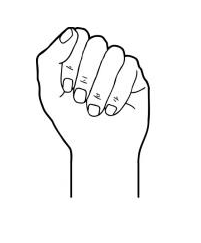
\includegraphics[width=\textwidth]{fist}
%                          \caption{Fist}
%
%                  \end{subfigure}%
%        \begin{subfigure}[b]{0.18\textwidth}
%                \centering
%                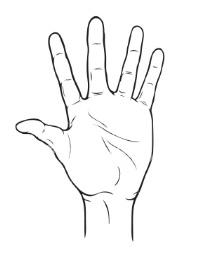
\includegraphics[width=\textwidth]{handopen}
%                \caption{Open hand (initial pose)}
%
%        \end{subfigure}
%        \\
%        \begin{subfigure}[b]{0.2\textwidth}
%                        \centering
%                        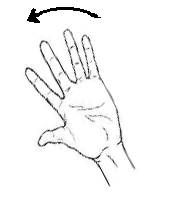
\includegraphics[width=\textwidth]{handleft}
%                        \caption{Rotate left}
%
%                \end{subfigure}
%       \begin{subfigure}[b]{0.21\textwidth}
%                        \centering
%                        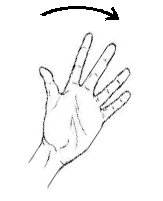
\includegraphics[width=\textwidth]{handright}
%                        \caption{Rotate right}
%
%                        \end{subfigure}
%        \begin{subfigure}[b]{0.25\textwidth}
%                        \centering
%                        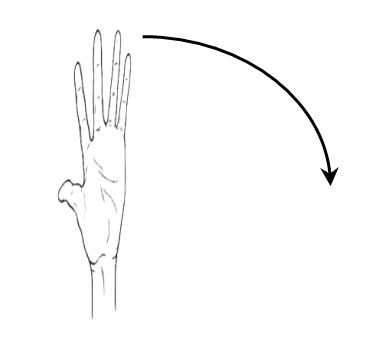
\includegraphics[width=\textwidth]{bendtofront}
%                        \caption{Bend down}
%
%                \end{subfigure}
%        \caption{Sample hand images: a) fist to stop motion, b) initial position (bottom), c) rotating left (upper left),  d) rotating hand right (upper right), e) bending hand down for acceleration (taken from \url{http://www.istockphoto.com})}\label{fig:gesture_images}
%\end{figure}
\section{Evaluation}
...
%The following test scenario will be used to test the performance of the library.
%Human operator puts his hand in front of the camera (gesture (2)) so that the plane of the hand is approximately perpendicular to the optical axis and its outline is confined within a rectangular working area depicted on the screen of the PC. When the hand is detected by the library, corresponding message is displayed on the PC's screen. The operator then bends the hand down and back and rotates it smoothly in the plane of the hand. Any part of the hand image should not move outside the allowed working rectangle.\\
%Possible evaluation task will be navigating the NXT robot along the specified path (e.g. drive 1 meter forward, then turn right, then move 2 meters forward). Navigating should be performed by user with no previous experience with the interface
%Possible issues:
%\begin{itemize}
%\item The hand is occluded from the camera by other objects or there are other objects with the same color as the hand within the working rectangular;
%\item The hand moves outside of the working rectangular;
%\item Lighting conditions change in such a way that the hand gestures and finger tracking cannot be performed accurately with predefined color model for the hand;
%\item The planar shape of the hand gesture (2) is not maintained quite precisely affecting estimation of the angles.
%\end{itemize}

\bibliographystyle{alpha}
\bibliography{bib}
\end{document}
